\section{Recurrent Models of Visual Attention}
\label{sec:ram_model}
As as it was mentioned in \autoref{chap:intro}, Recurrent Models of Visual
Attention(also known as the recurrent attention model(RAM)) is
a computational approach presented by google Deepmind’s researchers to reduce
and contronl computational cost while classifying images.
\subparagraph{Note: } The theory described in this section based on the
\cite{Ba2015}, unless otherwise stated.

\paragraph{Why RAM?}
Today's state of the art approaches to classify the images is convolutional
neural network(CNN). Nevertheless, to train CNN model on the high resolutional
images will require days of time. Similar to RNN models, some computations
in CNN are shared, however the main cost is laid on applying the convolutional
filter on the entire image, hence the bigger image is the
more computations is required.\cite{Krizhevsky2012}

Recurrent model attention is trying to face this problem by
controlling amount of computations by adaptively selecting a sequence of
locations and only processing these location at high-resolution


\paragraph{The reccurent attention model}
The attention problem in RAM is considered as sequential decision
process of an agent who interact with visual environment. The idea is,
that agent never sees the whole input, but only receives the observations
via bandwidth-limited sensor. The goal for our agent is
to find and select those locations on the images where the agent can extract
most of information needed for a classification decision.
To summarize it:
\begin{itemize}
	\item Agent selects a location on the image
	\item Agent receives an observation
	\item Agent extracts the information from the observation via bandwidth-limited
		sensor with respect to the location.
	\item Based on what he extracted, he selects the next location.
	\item If current time step is
		more than some predefined number $T$, agent is forced to do a
		classification decision.
\end{itemize}

\begin{figure}[H]
	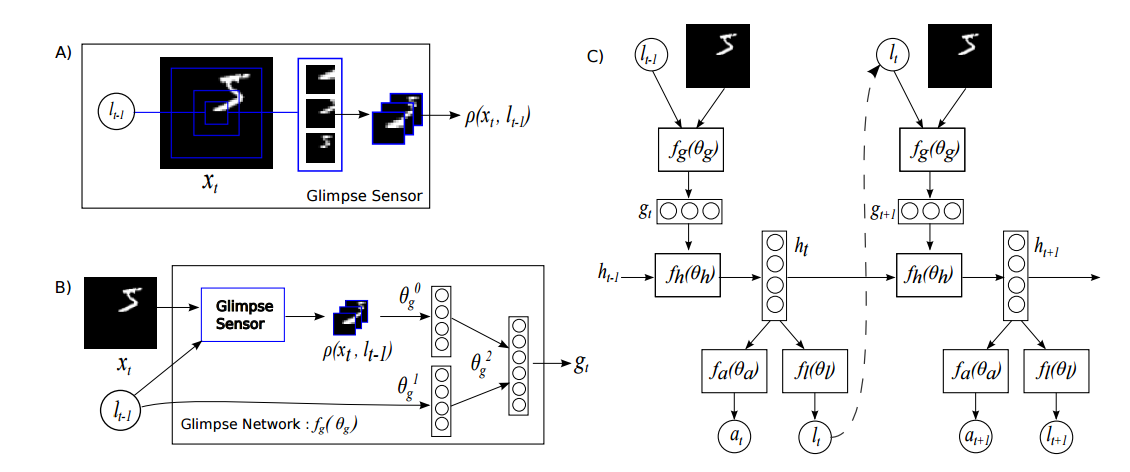
\includegraphics[width=\linewidth]{ram_model.png}
	\caption{
		A) Glimpse Sensor,
		B) Glimpse Network,
		C) Model Architecture,
		(Source: \cite{Ba2015})
	}
	\label{img:ram_model}
\end{figure}

In figure \ref{img:ram_model}, you can see
\emph{glimpse sensor}, \emph{glimpse network}, and the whole architecture
of the model.

\paragraph{Glimpse sensor} Glimpse sensor is formally the bandwidth-limited sensor
which takes image and location as input and produces the bandwidth-limited representation of it.
Thus, the main responsibility of the glimpse sensor
is to build from an image $x_t$ the image representation $\rho(x_t, l_{t-1})$
with respect to the location $l_{t-1}$. The sensor select a number of patches
 from an image $x_t$ centered at the location $l_{t-1}$ as you can see in \ref{img:ram_model}.
 The first batch is processed at high resolution, while for patches further
 from $l_{t-1}$, progressively lower resolution is used. This representation contained
 multiple resolution patches
 of an image is known as \emph{glimpse} and is denoted as $\rho(x_t, l_{t-1})$. \cite{Larochelle2010}
 The glimpse sensor is used within glimpse network to produce
  glimpse feature vector.



%
% It encodes the region around l at a high-resolution but uses a progressively
% lower
% resolution for pixels further from l, resulting in a vector of much
%
% lower dimensionality than the original image x. We will refer to
% this low-resolution representation as a glimpse
%
% The glimpse sensor is used inside what we call the glimpse network
% fg to produce the glimpse feature vector


\paragraph{Glimpse network} As you can see in figure \ref{img:ram_model} B),
glimpse network takes an image $x_t$ and
location $l_{t-1}$ as an input and produces the glimpse feature vector
$g_t = f_g (x_t, l_{t-1}; \theta_g)$. Glimpse network uses glimpse sensor to
create a glimpse $\rho(x_t, l_{t-1})$. Then it feeds this glimpse and the location
$l_{t-1}$ into two independent neural networks with parameters $\theta_g^0$ and $\theta_g^1$
respectively followed by another neural network which combines the information
from both components. The last NN parametrized by $\theta_g^2$ produces then
final feature vector $g_t = f_g (x_t, l_{t-1}; \theta_g)$,
where $\theta_g = \{\theta_g^0, \theta_g^1, \theta_g^2\}$.

\paragraph{Model Architecture} The model architecture is shown
on picture C) in the figure \ref{img:ram_model}. The agent is built around
the RNN and uses RNN's output as internal state. RNN's output $h_t$ contains
information from past glimpses and locations. It's possible
because the RNN at each time step $t$ receives $g_t$ as external input and
summarizes it by using a LSTM cell : $h_t = f_h(h_{t-1}, g_t; \theta_h)$.

\subparagraph{Actions} Agent perfumes two types of actions: environment actions
and location action. Location action $l_t$ decides where to allocate the next glimpse
on the picture. The location network $f_l(h_t; \theta_l)$ is a NN layer
that produces the next location $l_t$ parametrized by $\theta_l$. We will consider the
location network a bit deeper in the \autoref{chap:analysis}. \\
Depends on the task, environment actions can vary, therefore
we'll concentrate on the environment action that is relevant for this work.
In our work, environment actions makes the classification decision of an image.
It's formulated using softmax output from environment neural network
 $f_a(h_t; \theta_a)$, where $\theta_a$ - is a parameter of neural network $f_a$.

\subparagraph{Rewards} As we making a classification decision only after $T$
number of steps, our reward signal will be delayed. Therefore agent is receiving
a reward $r_n = 1$ if the classification decision was correct and $0$ otherwise.


Training of the agent is performed by REINFORCE rule described in \autoref{ss:pol_based_rl}.
% Given the location (lt−1) and input image (xt), uses the glimpse sensor to extract
% retina representation ρ(xt, lt−1). The retina representation and glimpse
% location is then mapped into a hidden space using independent linear
% layers parameterized by θ0
% g and θ1 g respec-
% tively using rectified units followed by another linear layer θ2
% g to combine the information from both components. The glimpse network
% fg(.; {θ0 g, θ1g, θ2g}) defines a trainable bandwidth limited sensor
% for the attention network producing the glimpse representation gt



% image

% explaining the image


% maybe explaining the state, reward, and etc.

% learning using reinforce rule



% adaptively selecting a sequence of regions or locations and only
% processing the selected regions at high resolution.
